%!TEX root = report.tex
In this section we will discuss the control flow in the front end upon certain actions of the user. To avoid a lengthy report we will only discuss the flow of successful cases.

\subsection{Log In}
\label{ss:1:login}
	As mentioned earlier users have to log in to a social network before being allowed to stalk somebody on that network. Since we store the ID of the user and we have not implemented an api call that adds for example the LinkedIn identification to a user that we have already stored with its Facebook identification.

	\Cref{fig:1:controlflowLogIn} presents the flow of control when a users logs in. The views that are presented to the user before and after logging in are presented in \cref{fig:1:viewLogIn}.

	The \t{loggedIn}, and its not shown equivalent \t{loggedOut}, event ensure that the \t{searchController} knows that a user is logged in. The \t{Facebook Service}, \t{ngFacebook}, is discussed \vref{ssec:1:angularjs}. 

	Logging out of social network is comparable to logging into it. \Cref{fig:1:controlflowLogIn} uses Facebook, the application works in exactly the same way for e.g. LinkedIn.

	\begin{figure}
		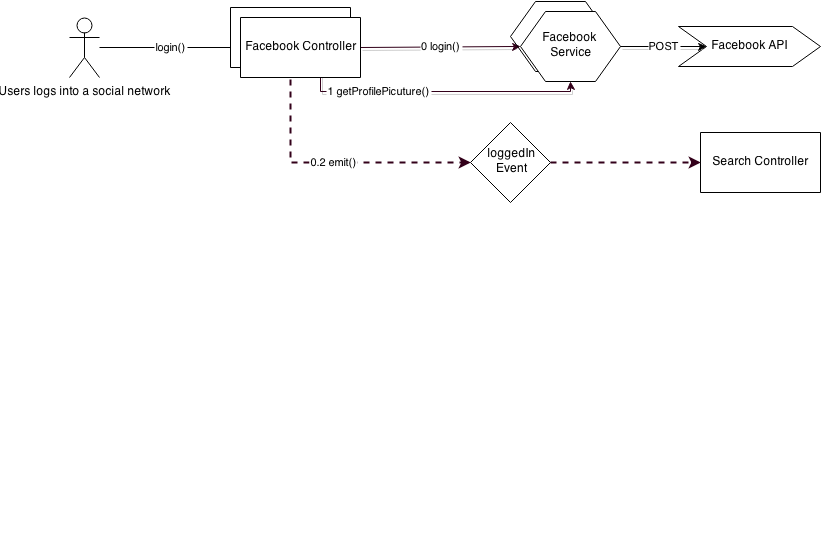
\includegraphics[width=\textwidth]{./img/1_login_flow}
		\caption{A schematic overview of the control flow when a user logs in.}
		\label{fig:1:controlflowLogIn}
	\end{figure}

	\begin{figure}
		\begin{subfigure}{\textwidth}
			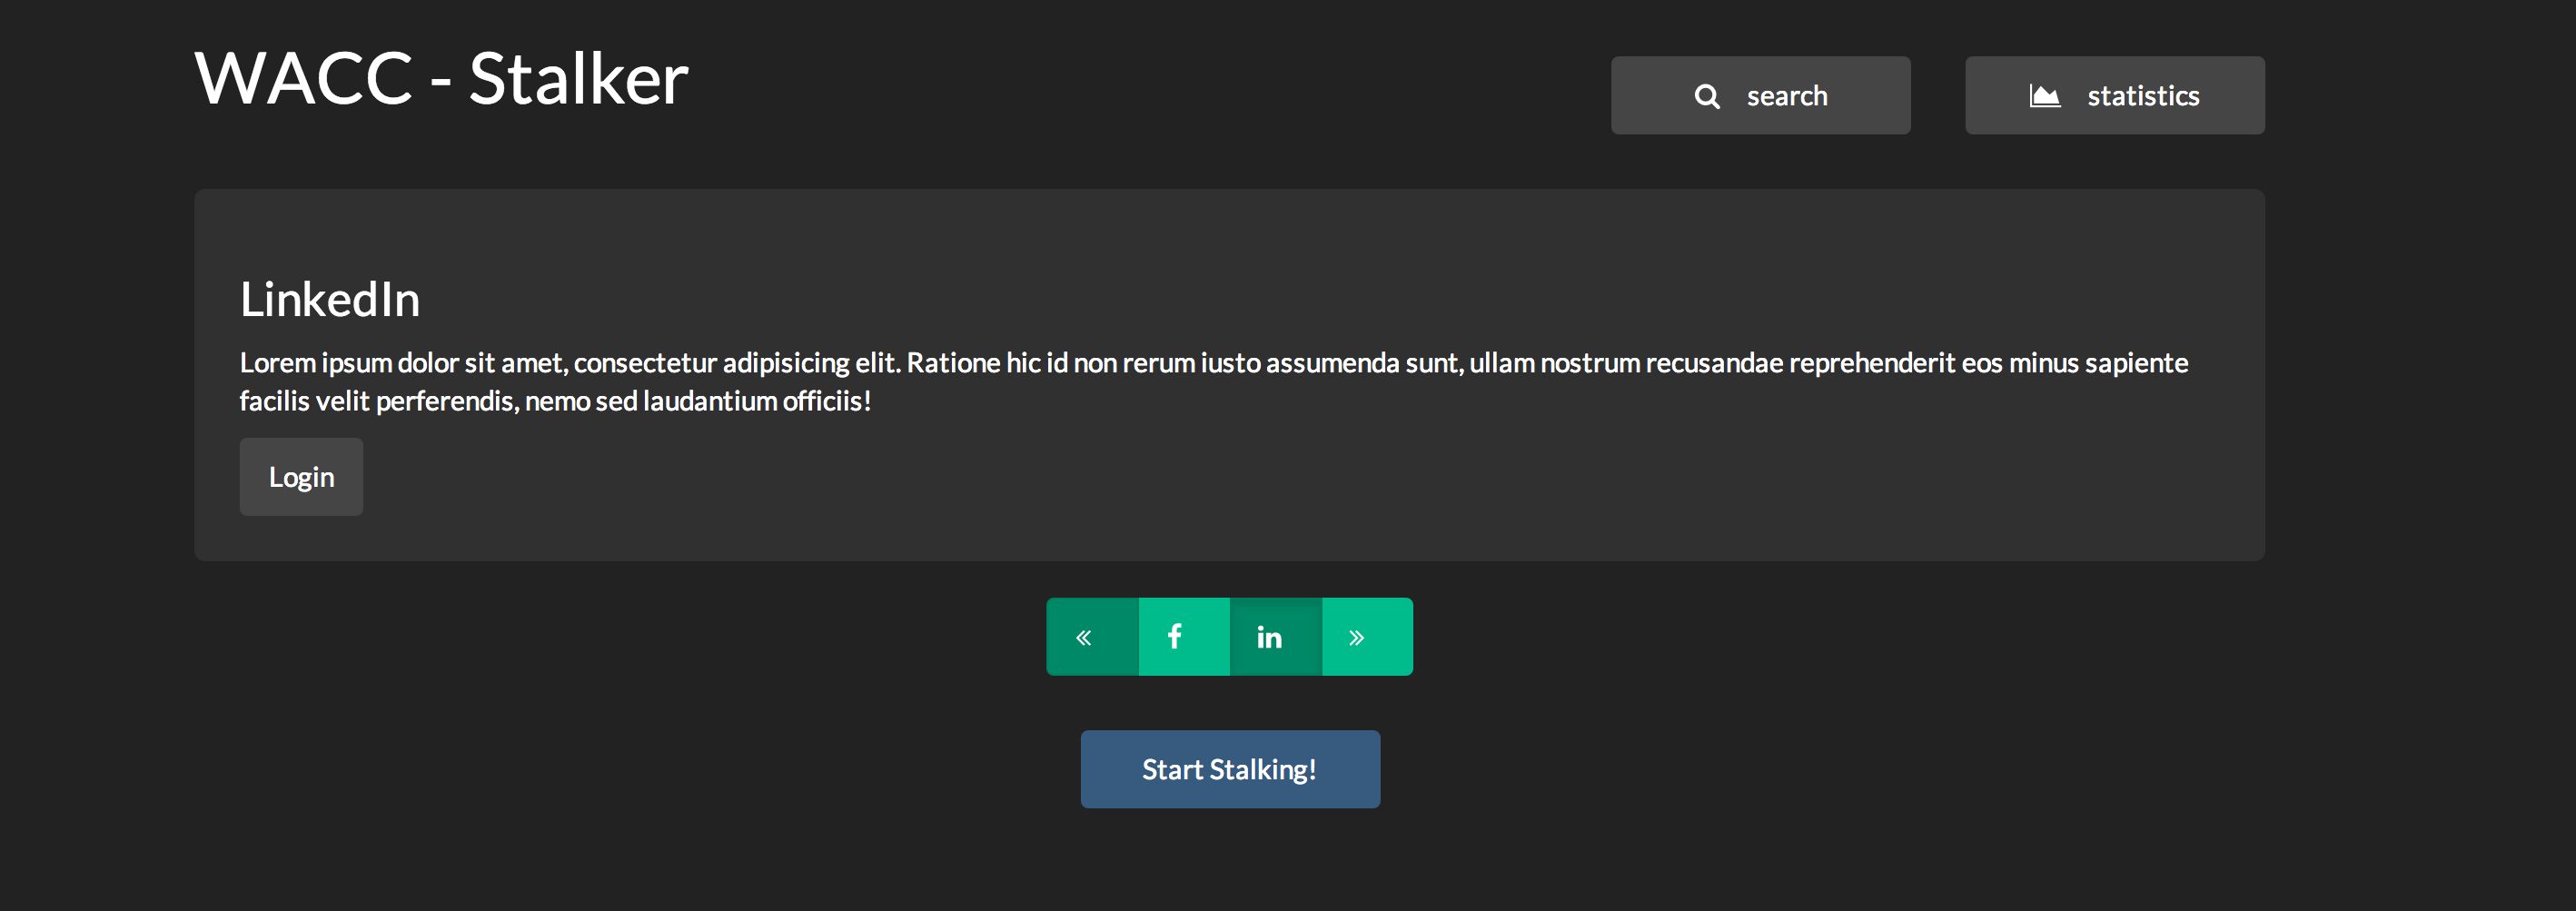
\includegraphics[width=\textwidth]{./img/1_login_view_logged_out}
			\caption{The view when the user is not logged into LinkedIn.}
			\label{fig:1:viewLogIn:linkedin}
		\end{subfigure}
		\begin{subfigure}{\textwidth}
			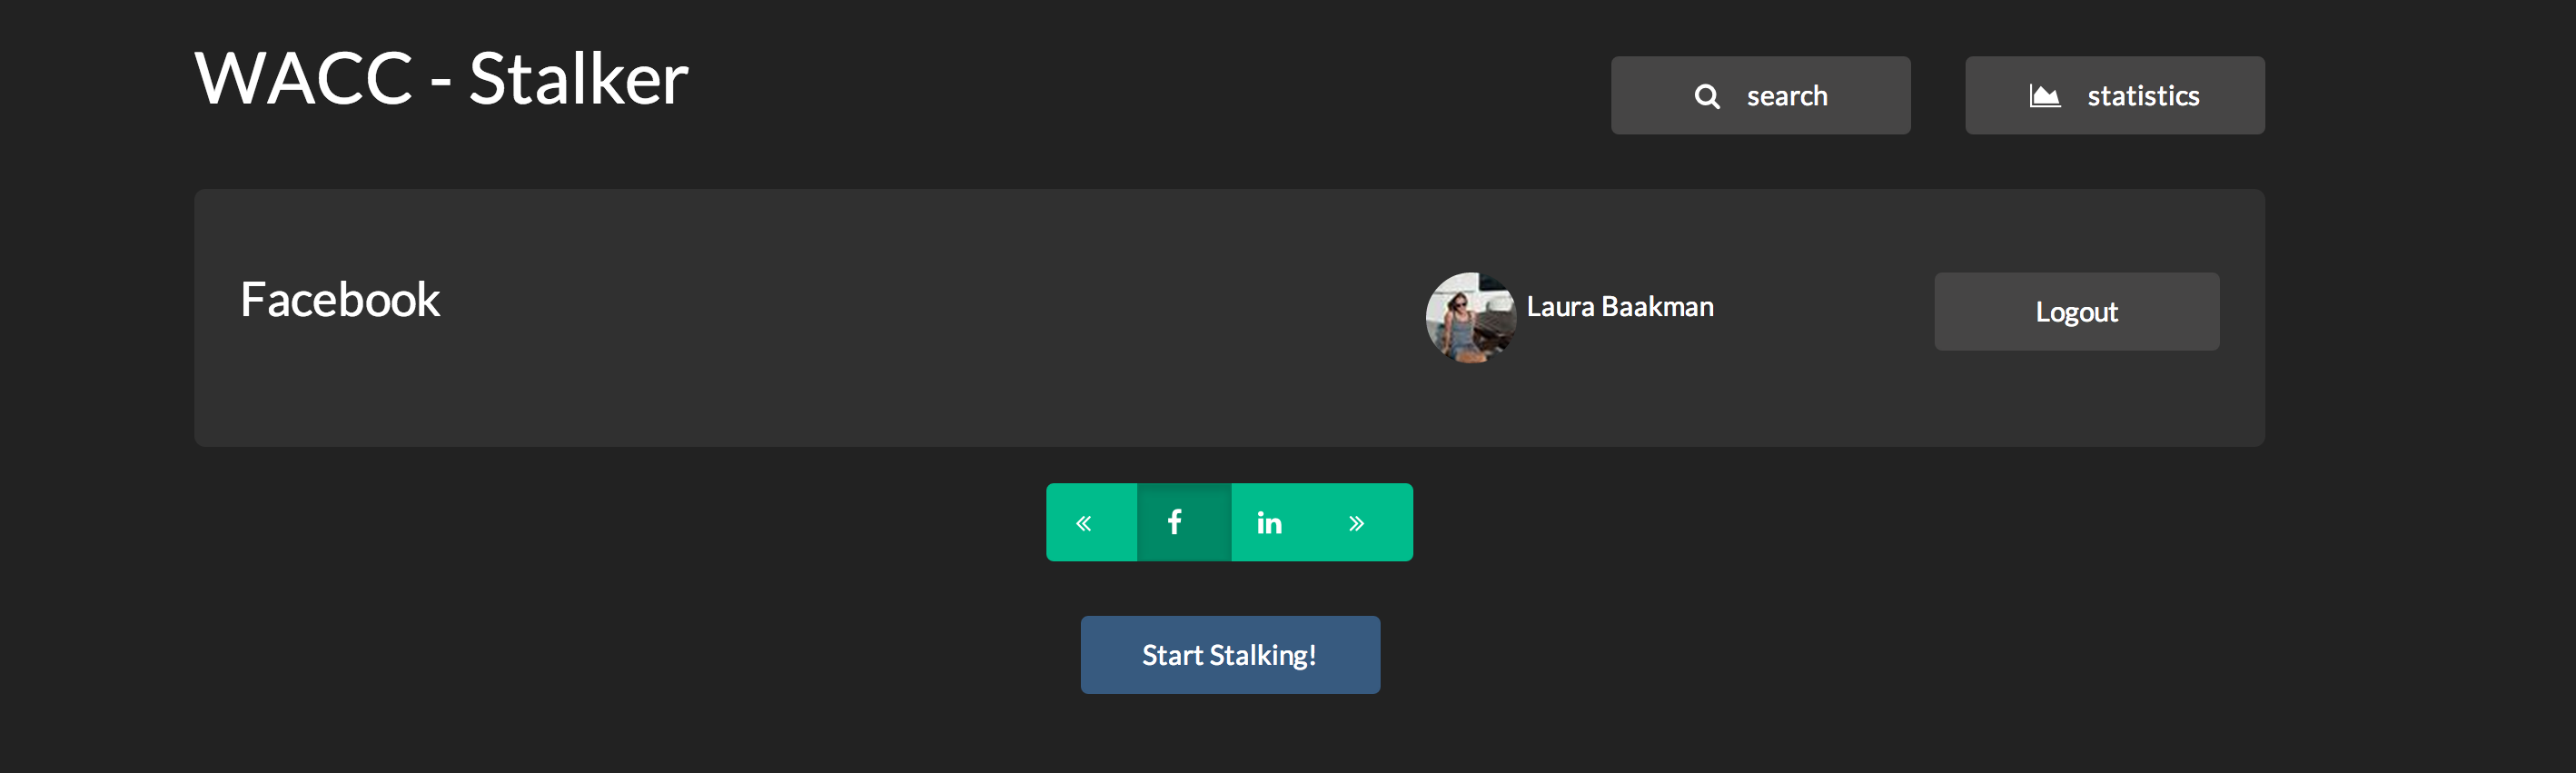
\includegraphics[width=\textwidth]{./img/1_login_view_logged_in}
			\caption{The view when the user is logged into Facebook.}
			\label{fig:1:viewLogIn:facebook}
		\end{subfigure}			
		\caption{Screen shots of the application when \subref{fig:1:viewLogIn:facebook} the user still has not yet logged into LinkedIn and \subref{fig:1:viewLogIn:linkedin} the user has logged in into Facebook.}
		\label{fig:1:viewLogIn}
	\end{figure}	

\subsection{Start Stalking}
\label{ss:1:startStalking}
	\Cref{fig:1:controlflowStartStalk} shows what happens in the front end when the button `start stalking', see \autoref{fig:1:viewLogIn}, is pressed. the \t{Stalker Service} contains all information on the stalker. The \texttt{API Service} contains all calls to our own API, we have chosen for a separate service so that we only have to store the address of the API in one place. The Search Service broadcasts the search to the different social media controllers, in \cref{fig:1:controlflowStartStalk} Facebook is shown as an example. Each social network controller does a search call by calling some function in the matching service that interacts with the actual API of that social network.


	We had to use a broadcast instead of an emit as in \cref{ss:1:login} since we had to down in the scope hierarchy instead of up. 

		\begin{figure}
			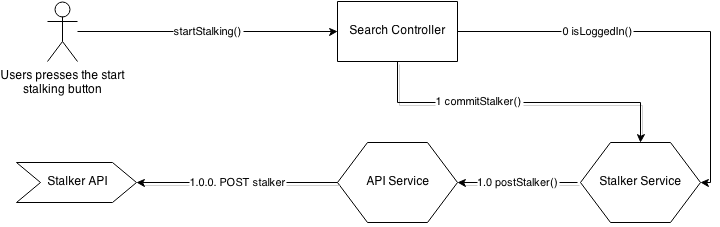
\includegraphics[width=\textwidth]{./img/1_start_stalking_flow}
			\caption{A schematic overview of the control flow when a presses the `start stalking' button.}
			\label{fig:1:controlflowStartStalk}
		\end{figure}


\subsection{Stalk}
	\Cref{fig:1:controlflowStalk} presents the flow of control when a user searches for somebody on the social networks that he has logged in to. The views presented to the user are shown in \autoref{fig:1:viewStalk}.

	\todo{Begeleidend verhaaltje schrijven}

		\begin{figure}
			\missingfigure{Control flow of stalking}
			\caption{A schematic overview of the control flow when a user stalks somebody.}
			\label{fig:1:controlflowStalk}
		\end{figure}	

		\begin{figure}
			\begin{subfigure}{\textwidth}
				\missingfigure{Screenshot of the application when a user has to start filled out data, and is about to press the stalk button.}
				\caption{The view when the user is about to press the stalk button.}
				\label{fig:1:viewStalk:startStalk}
			\end{subfigure}
			\begin{subfigure}{\textwidth}
				\missingfigure{Screenshot with a list of results.}	
				\caption{The view when all victims are found.}
				\label{fig:1:viewStalk:allVictims}
			\end{subfigure}		
			\begin{subfigure}{\textwidth}
				\missingfigure{Screenshot with a one result}	
				\caption{The view with the details of one victim.}
				\label{fig:1:viewStalk:oneVictim}
			\end{subfigure}						
			
			\caption{Screen shots of the application when \subref{fig:1:viewStalk:startStalk} the user is about to press the stalk button, \subref{fig:1:viewStalk:allVictims} the list of all victims, \subref{fig:1:viewStalk:oneVictim} the details of one victim.}
			\label{fig:1:viewStalk}
		\end{figure}

\subsection{Select Victim}
	\Cref{fig:1:controlflowVictim} shows the control flow in the front end when a user indicates that one of the found results was his victim. The view presented to the user upon successfull submission of his victim is presented in \cref{fig:1:viewVictim:selectedVictim}.

		\begin{figure}
			\missingfigure{Control flow of choosing a victim}
			\caption{A schematic overview of the control flow when a user selects somebody as his victim.}
			\label{fig:1:controlflowVictim}
		\end{figure}	

		\begin{figure}
				\missingfigure{Screenshot of the application when a user has selected a victim.}
				\caption{The view when the user has selected a victim.}
				\label{fig:1:viewVictim:selectedVictim}
		\end{figure}	

\subsection{View Statistics}
	The control flow when a user views statistics is presented in \cref{fig:1:controlflowStat}. \Cref{fig:1:viewStat} shows how the statistics are presented to the user.

	\todo{Begeidend verhaaltje schrijven}

	\begin{figure}
		\missingfigure{Control flow of statistics}
		\caption{A schematic overview of the control flow of requesting the statistics and showing them to the user.}
		\label{fig:1:controlflowStat}
	\end{figure}

	\begin{figure}
		\missingfigure{View statistics}
		\caption{The view when the user has requested statistics.}
		\label{fig:1:viewStat}
	\end{figure}